%% osm-fonctionnement.tex
%%


\section{Fonctionnement}

\frame[plain]{  \heading{Plan de la Présentation}
\ecmsetupplan
\begin{itemize}
  \item[\small $\Diamond$] Introduction
  \item[\small $\Diamond$] {\color{purple}\textbf{Fonctionnement}}
  \item[\small $\Diamond$] Démonstration
  \item[\small $\Diamond$] Applications
  \item[\small $\Diamond$] Conclusions
\end{itemize}
}


\frame { \heading{Fonctionnement} \vfill

  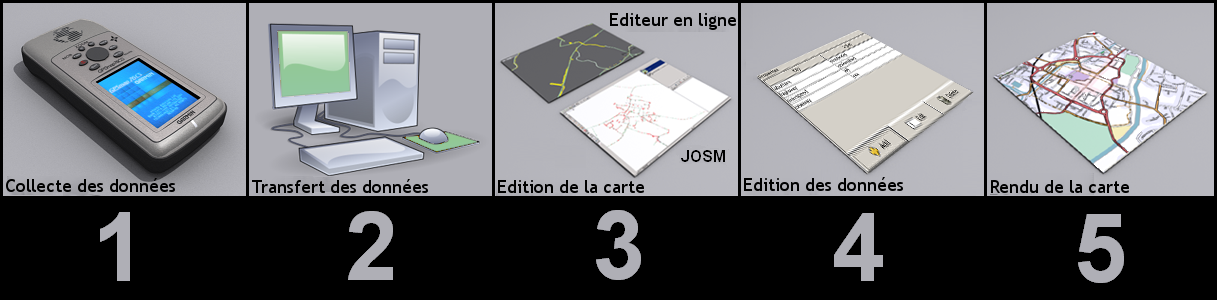
\includegraphics[width=\textwidth]{figures/OSM-steps}

  \begin{enumerate}
  \item Collecter les données
  \item Transférer les données GPS
  \item Générer et éditer les données OSM
  \item Ajouter des labels et des méta-data
  \item Exploiter les données (générer un rendu)
  \end{enumerate}
}


\frame { \heading{Collecte des données}
  \begin{tikzpicture}[remember picture,overlay]
   \node[xshift=-1cm,yshift=-1.3cm] at (current page.north east) {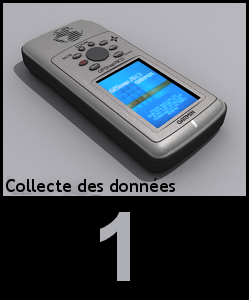
\includegraphics[width=2cm]{figures/OSM-step1}};
  \end{tikzpicture}

  Sources de données:
  \begin{itemize}
  \item logs GPS crées à pied, à vélo, en voiture, en train, avec notes et photos du trajet
  \item Cadastre numérique (en France)
  \item photos satellite Yahoo! (dans les zones couvertes)
  \item CORINE land cover (en Europe)
  \item imagerie satellite Landsat 7
  \item TIGER (aux USA)
  \item AND (Pays Bas, Chine, Inde)
  \end{itemize}

  \bigskip
  {\Large\color{red}\Stopsign{}} Interdiction d'utiliser les cartes propriétaires!
}


\frame { \heading{Transfert des données}
  \begin{tikzpicture}[remember picture,overlay]
   \node[xshift=-1cm,yshift=-1.3cm] at (current page.north east) {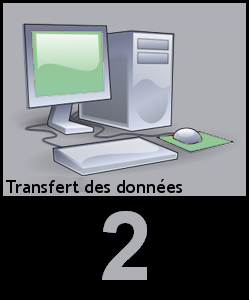
\includegraphics[width=2cm]{figures/OSM-step2}};
  \end{tikzpicture}

  \begin{itemize}
  \item Transférer les données vers l'ordinateur
  \item Conversion au format GPX et suppression points redondants
    \begin{itemize}
    \item outil: GPSBabel
    \end{itemize}
  \item Upload des tracks vers OSM via le site web
    \begin{itemize}
    \item nécessite un compte openstreetmap
    \end{itemize}
  \end{itemize}
}


\frame { \heading{Édition de la carte}
  \begin{tikzpicture}[remember picture,overlay]
   \node[xshift=-1cm,yshift=-1.3cm] at (current page.north east) {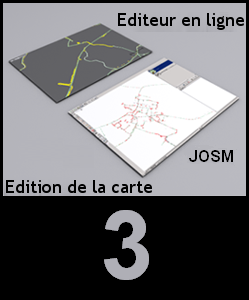
\includegraphics[width=2cm]{figures/OSM-step3}};
  \end{tikzpicture}


  \begin{itemize}
  \item Générer et éditer les n\oe{}uds et ways dans OSM
  \item Édition en ligne avec Potlatch (application Flash)
  \item Édition hors-ligne avec JOSM (application Java)
  \item Autres logiciels et scripts d'édition
    \begin{itemize}
    \item import massif de données (ex: Corine)
    \end{itemize}
  \item API REST permettant de développer d'autres applications
  \end{itemize}
}

\frame { \heading{Édition des données}
  \begin{tikzpicture}[remember picture,overlay]
   \node[xshift=-1cm,yshift=-1.3cm] at (current page.north east) {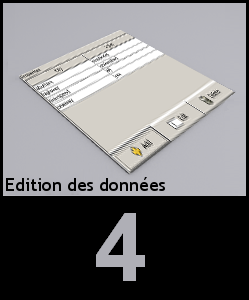
\includegraphics[width=2cm]{figures/OSM-step4}};
  \end{tikzpicture}

  \begin{itemize}
  \item Ajouter des étiquettes et méta-données
  \item Ajouter des données aux n\oe{}uds et ways pour permettre leur rendu
  \item Outils d'édition: JOSM, Potlatch
  \item Outils de détection d'incohérences:
    \begin{itemize}
    \item plugin <<validator>> pour JOSM
    \item couche <<maplint>> des cartes
    \item outils en ligne comme Keepright!, Osmose
    \end{itemize}
  \end{itemize}
}


\frame { \heading{Rendu de la carte}
  \begin{tikzpicture}[remember picture,overlay]
   \node[xshift=-1cm,yshift=-1.3cm] at (current page.north east) {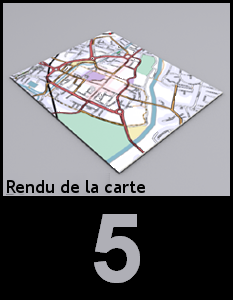
\includegraphics[width=2cm]{figures/OSM-step5}};
  \end{tikzpicture}

  \begin{itemize}
  \item Se fait automatiquement une fois que les données sont transférées
    vers le serveur

  \item Application Mapnik
    \begin{itemize}
    \item pré-traitement avec PostGIS pour accélérer le rendu
    \item rendu mis à jour en quelques heures
    \end{itemize}

  \item Application Osmarender (pipeline XSLT)
    \begin{itemize}
    \item possiblité d'utiliser des feuilles de styles XSLT personnalisées pour
      obtenir des cartes spécialisées
    \item possibilité d'exporter les cartes vers du SVG pour retouche manuelle
    \end{itemize}

  \item Visualisation des tuiles depuis une interface web (Slippymap)
    ou depuis applications spécialisées comme Viking
  \end{itemize}
}

% \frame { \hfill 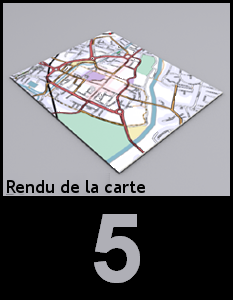
\includegraphics[width=2cm]{figures/OSM-step5}
% 
%   %% http://wiki.openstreetmap.org/wiki/List_of_OSM_based_Services
%   Plusieurs jeux de tuiles spécialisés existent:
%   \begin{itemize}
%   \item \href{http://www.opencyclemap.org/}{OpenCycleMap.org}, pistes cyclables, avec topographie
%   \item \href{http://www.openpistemap.org/}{OpenPisteMap.org}, carte des pistes
%   \item \href{http://www.öpnvkarte.de/}{öpnvkarte.de}, transports en commun
%   \item \href{http://www.openseamap.org/}{OpenSeaMap.org}, navigation en mer
%   \item \href{http://www.osm-wms.de/}{WMS OSM}, services de mesurage 
%   \end{itemize}
% }



\frame{\centering OpenCycleMap.org\newline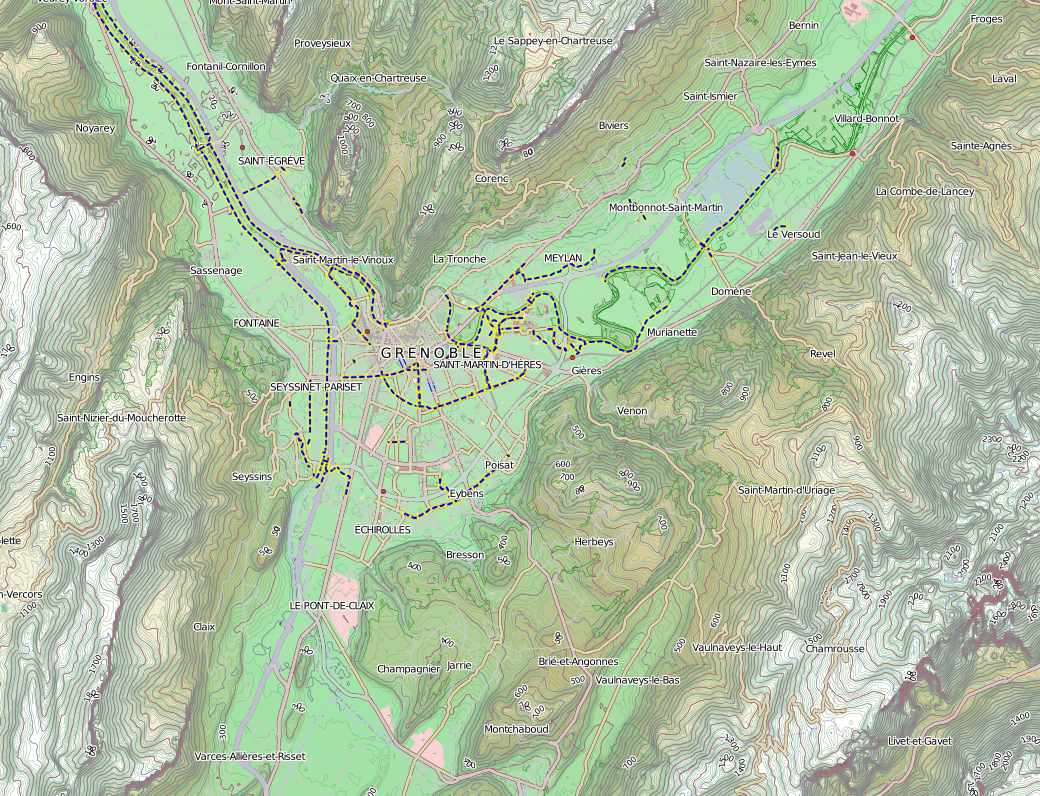
\includegraphics[width=0.95\textwidth]{figures/open-cycle-map}}
\frame{\centering OpenPisteMap.org\newline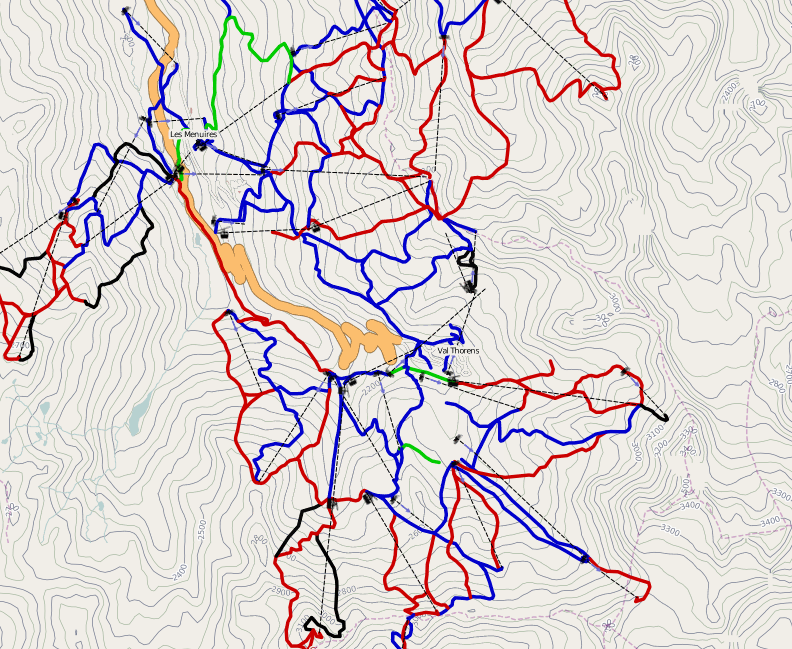
\includegraphics[height=0.94\textheight]{figures/open-piste-map}}
\frame{\centering öpenvkarte.de\newline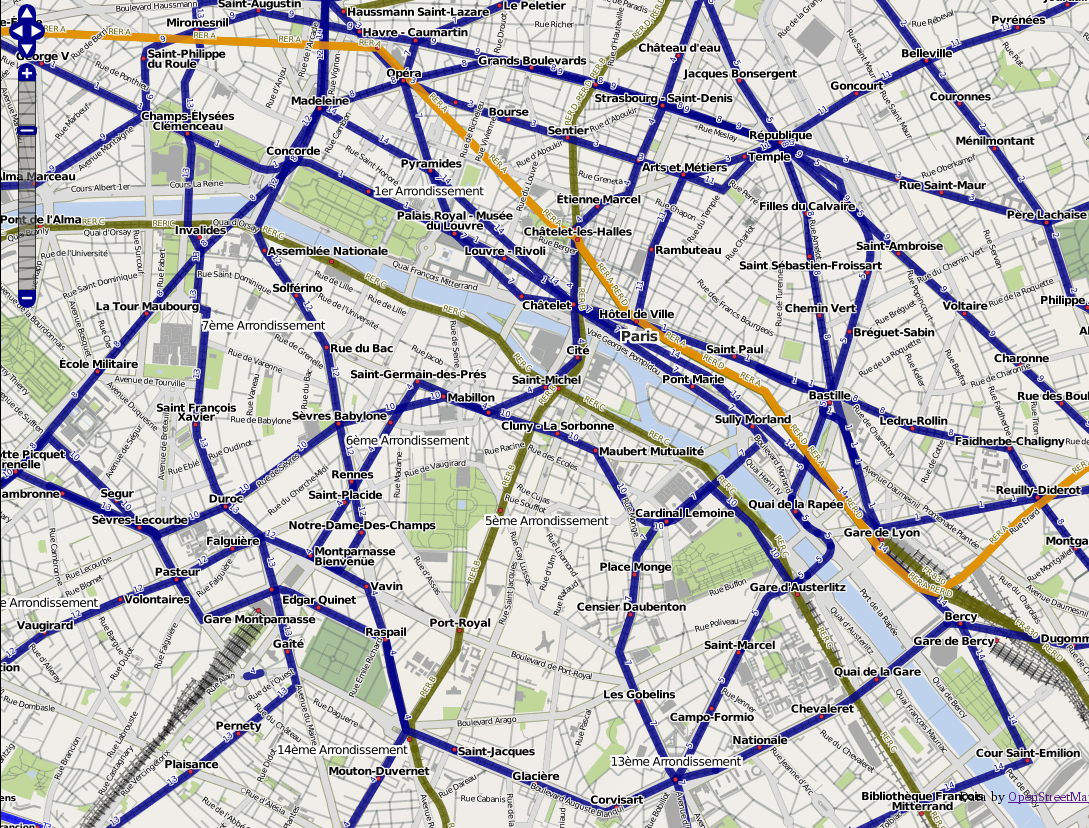
\includegraphics[width=0.98\textwidth]{figures/opnvkarte}}
\frame{\centering OpenSeaMap.org\newline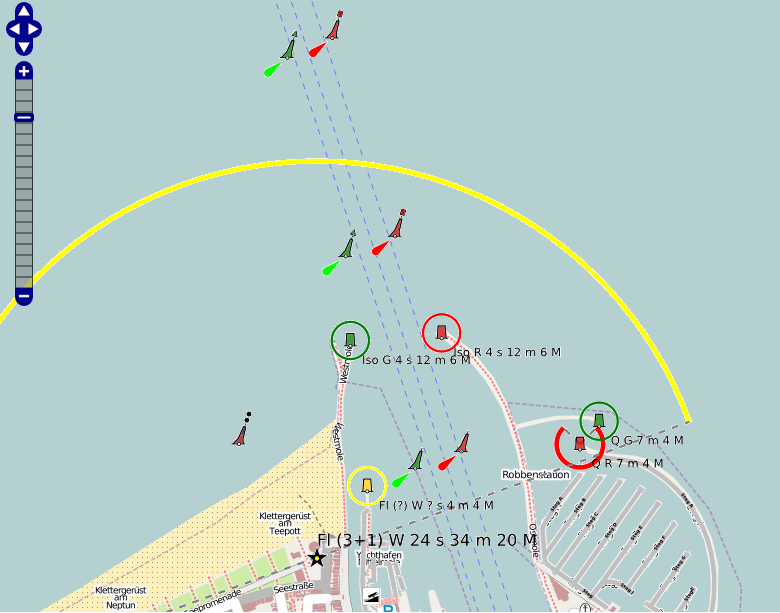
\includegraphics[width=0.98\textwidth]{figures/open-sea-map}}
\frame{\centering osm-wms.de\newline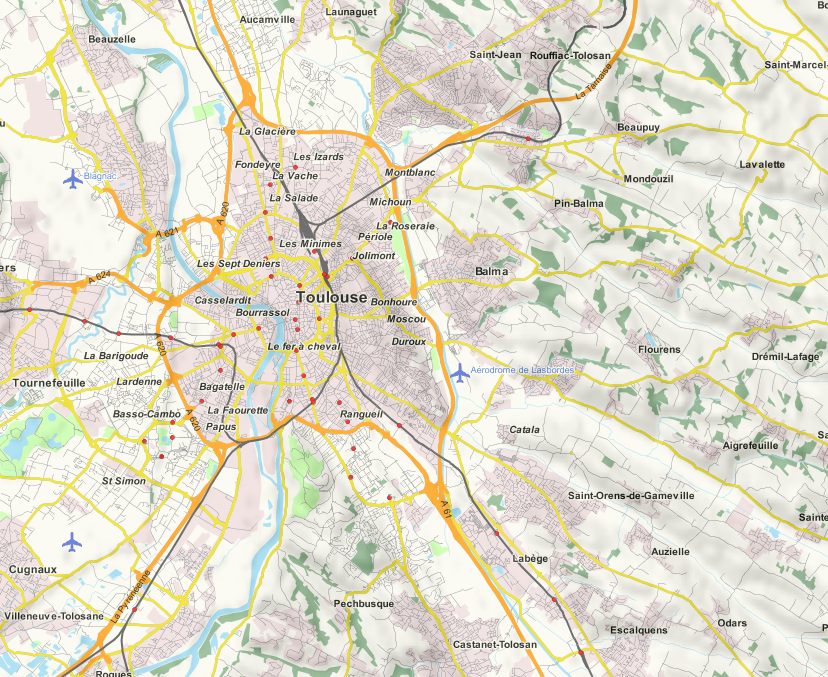
\includegraphics[width=0.98\textwidth]{figures/OSM-WMS}}
\frame{\centering TopOSM.com\newline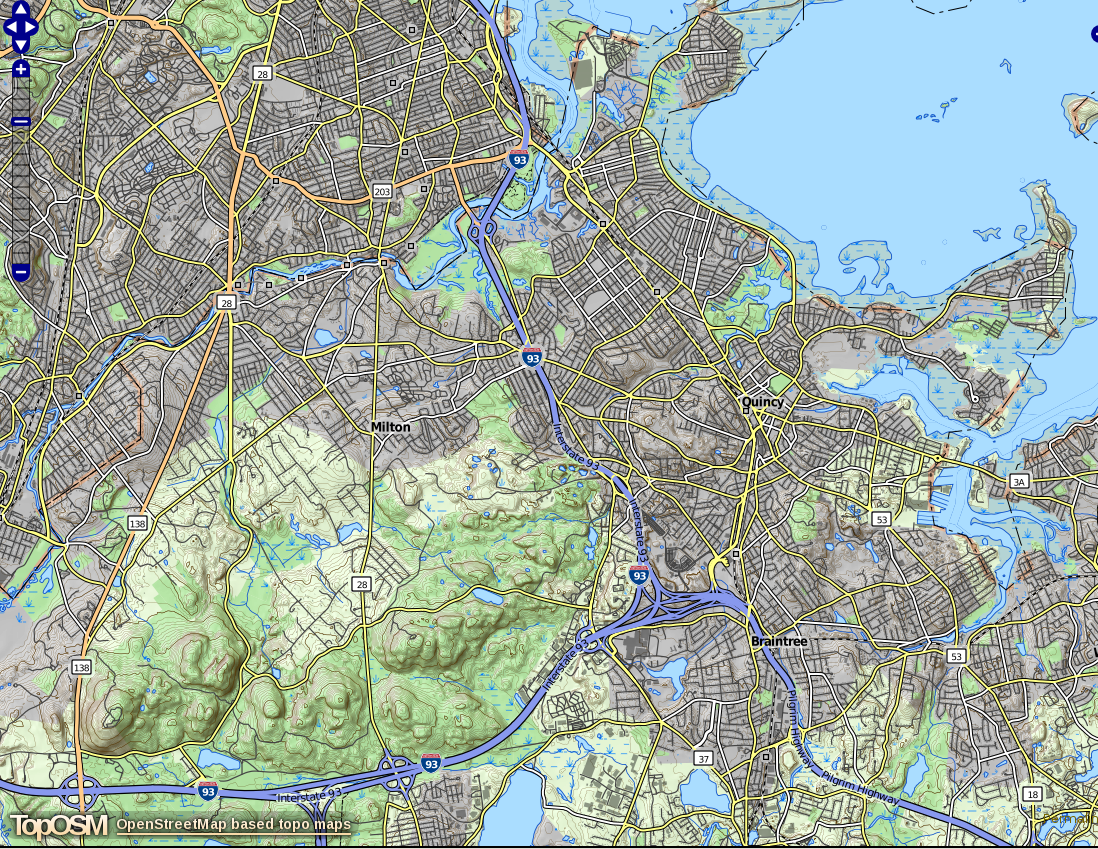
\includegraphics[width=0.99\textwidth]{figures/toposm}}




% \frame{ \heading{Structuration technique} \vfill
% 
% Structures de données employées:
% \begin{itemize}
% \item Un \textit{n\oe{}ud} est un point représentant une position
% \item Un \textit{way} (ou chemin) est une séquence de n\oe{}uds,
%   représentant une polyligne ou un polygône
% \item Une \textit{relation} est un ensemble de n\oe{}uds et de ways
%   auxquels on donne des propriétés 
% \item Une \textit{étiquette} ou tag peut être appliquée à un n\oe{}ud, un
%   way ou une relation, et consiste de paires \texttt{nom=valeur}
% \end{itemize}
% 
% \bigskip
% La sémantique des étiquettes est \href{http://wiki.openstreetmap.org/index.php/Map_Features}
% {décrite sur un wiki}. 
% }

\frame { \heading{Modèle de données} \vfill

  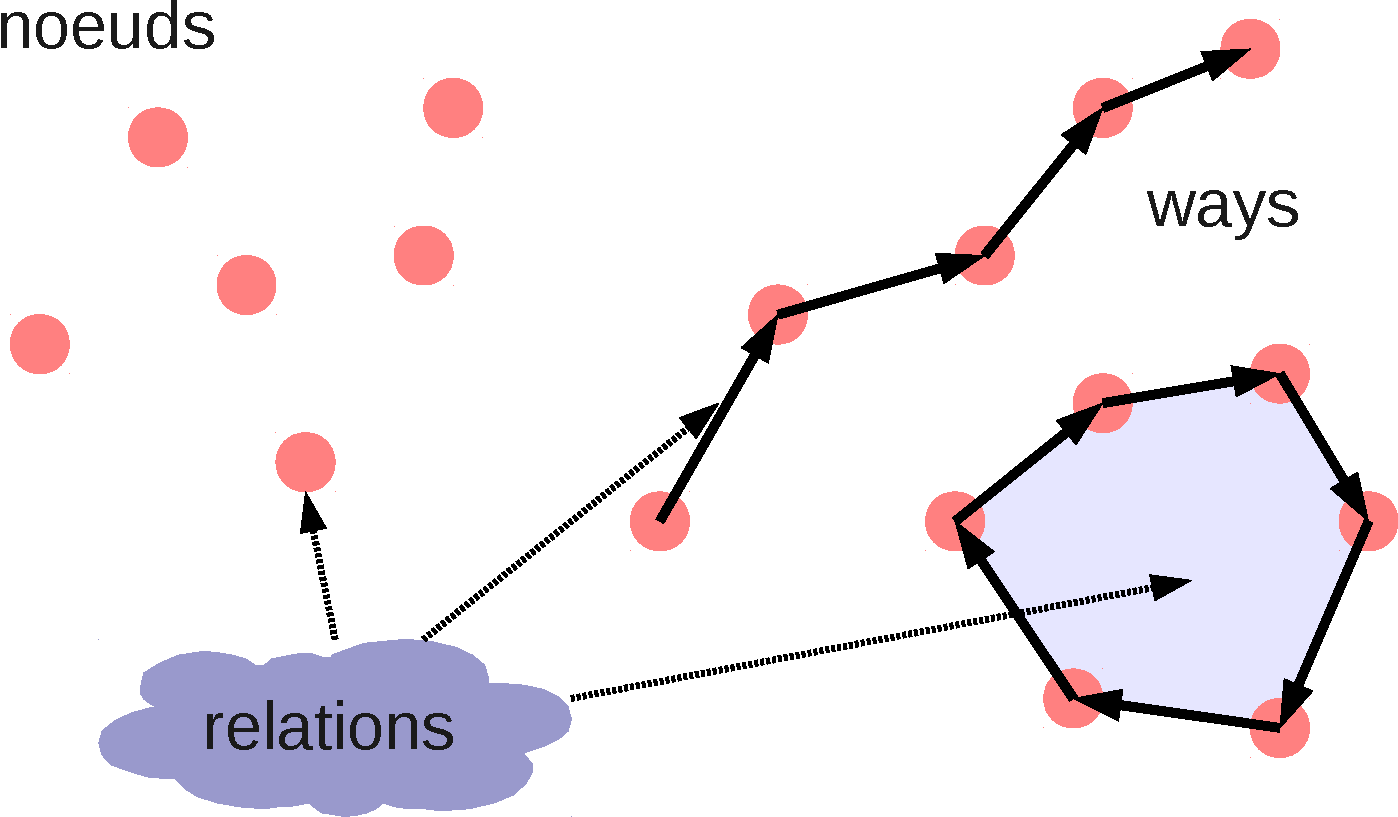
\includegraphics[width=0.95\textwidth]{figures/datamodel}
}


% http://wiki.openstreetmap.org/index.php/Map_Features
\frame{ \heading{Étiquettage} \vfill

  %% FIXME extract map in PDF format for better legibility
  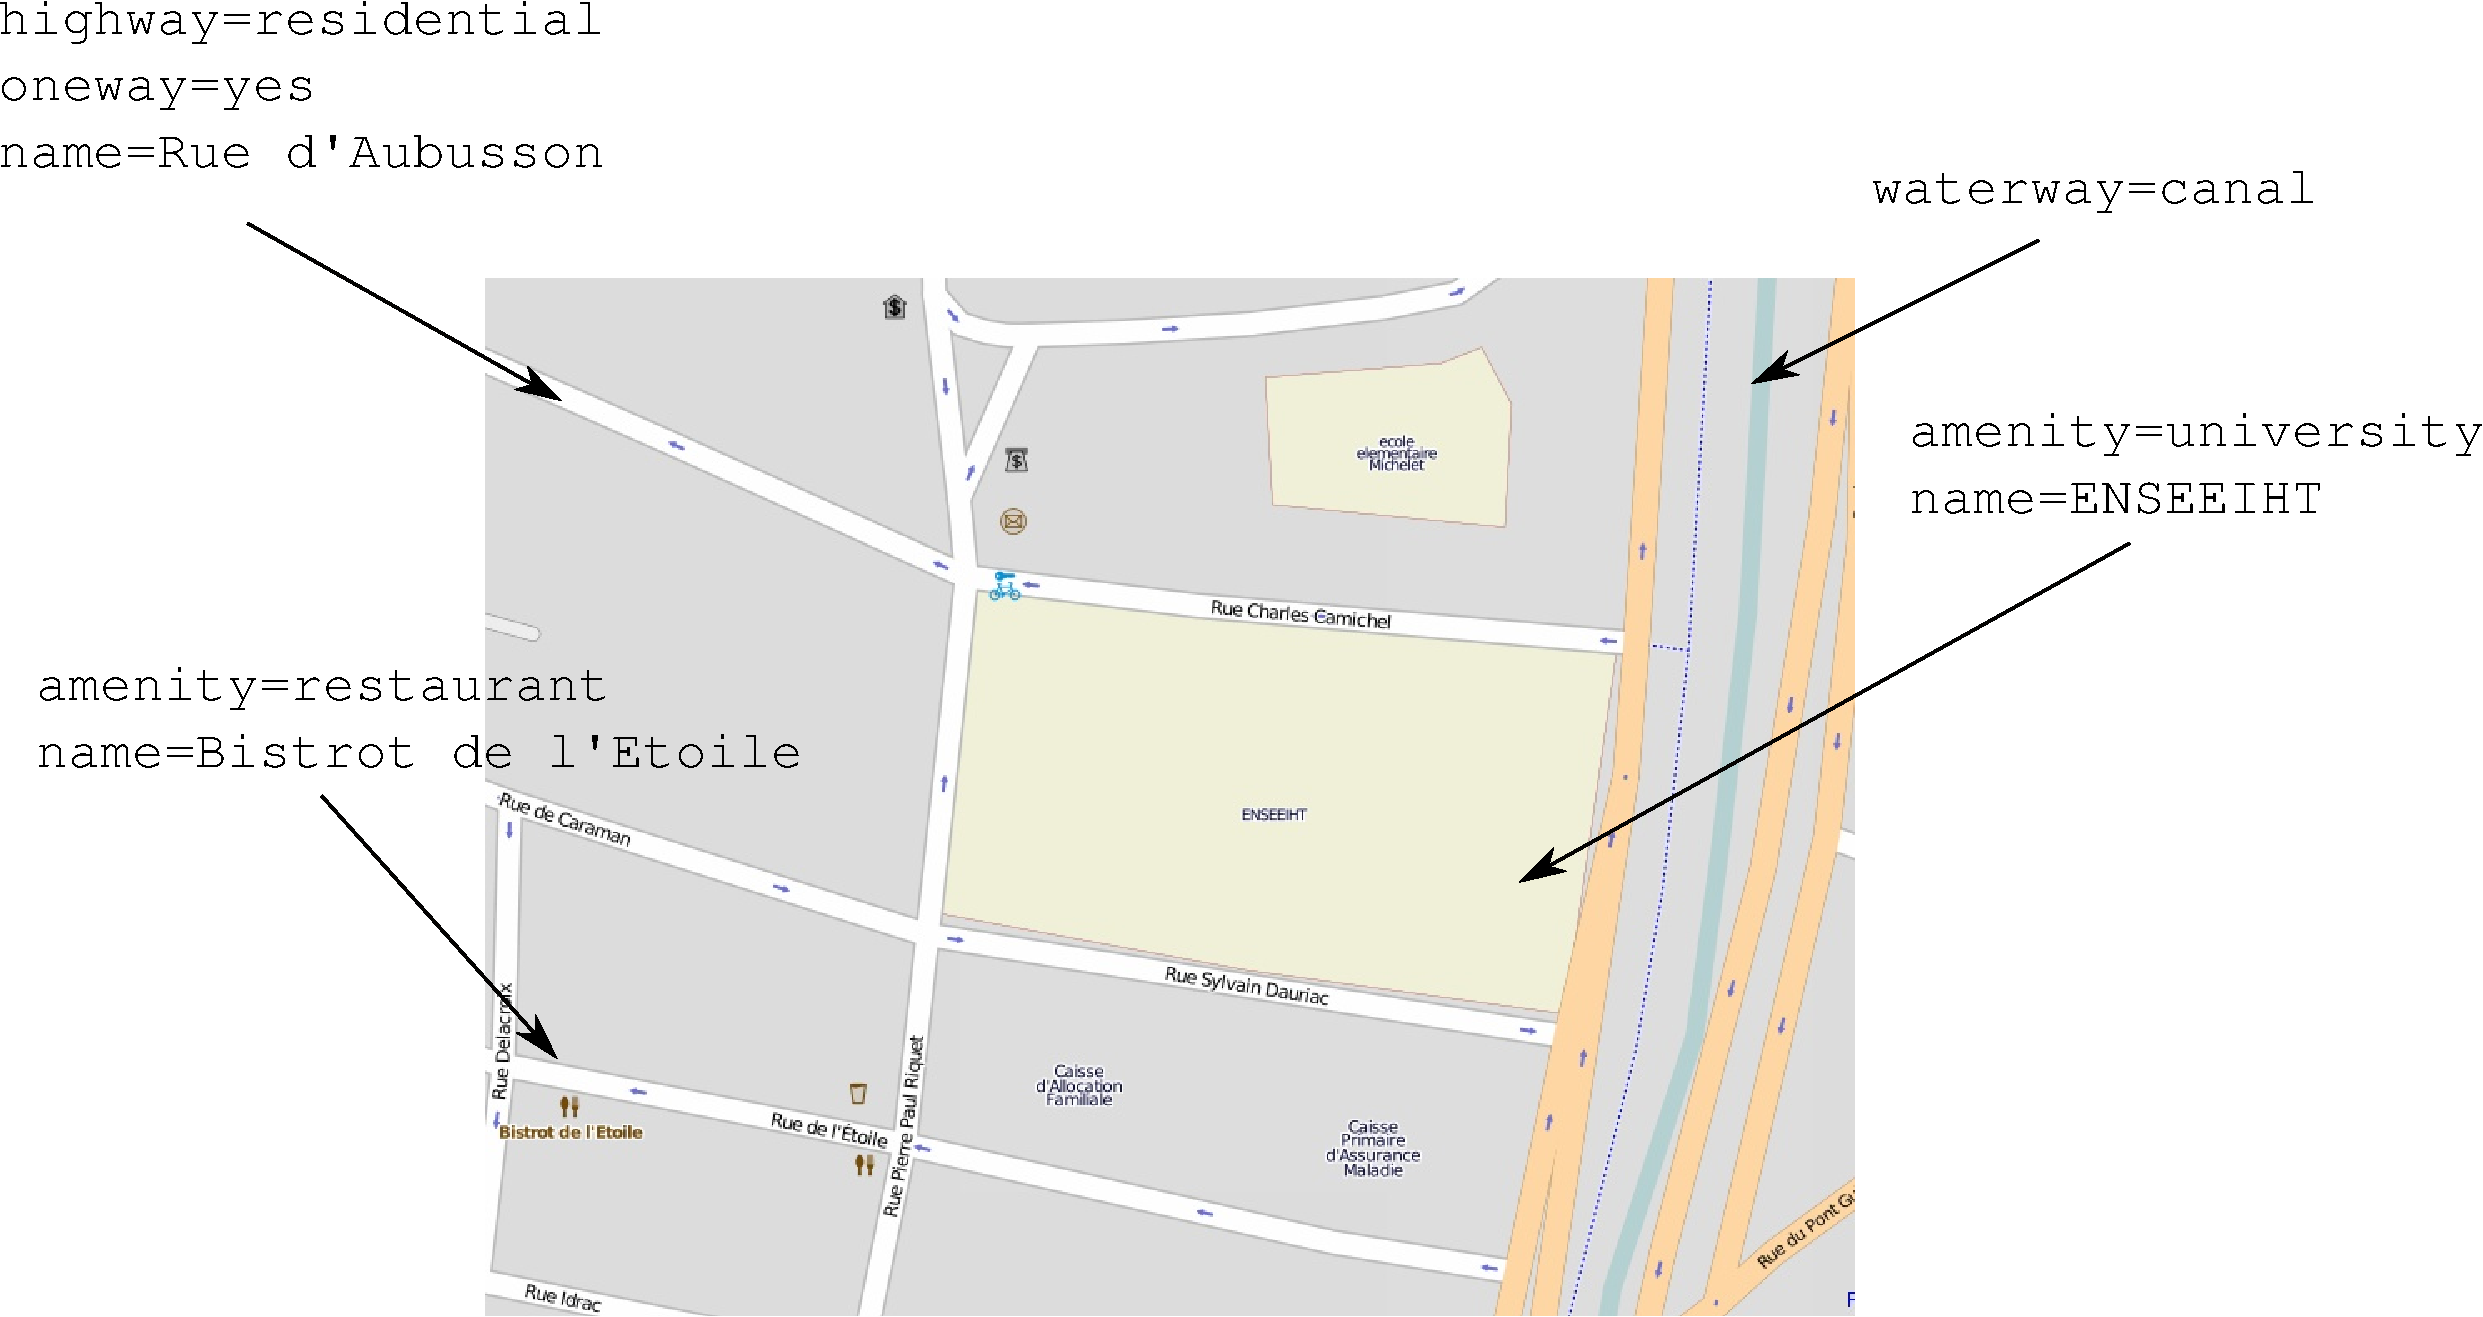
\includegraphics[width=0.99\textwidth]{figures/osm-tagging}

   {\footnotesize\textit{c.f.} \url{http://wiki.openstreetmap.org/index.php/Map\_Features}}
}
  
%   Exemples:
%   \begin{itemize}
%   \item highway = motorway
%   \item junction = roundabout
%   \item oneway = yes
%   \item cycleway = lane
%   \item waterway = canal
%   \item railway = station
%   \item railway = subway
%   \item leisure = park
%   \item amenity = pub
%   \item shop = supermarket
%   \item tourism = zoo
%   \end{itemize}



%% EOF
